\documentclass[sigconf,anonymous,review]{acmart}
\settopmatter{printacmref=false}
\setcopyright{none}
\renewcommand\footnotetextcopyrightpermission[1]{}
\acmConference[ICAIF '26 Workshop]{Workshop on Financial AI Security, Privacy and Safety at ICAIF 2026}{November 2026}{Milan, Italy}
\usepackage{graphicx}
\usepackage{booktabs}
\newcommand{\stcUnique}{15}
\newcommand{\stcTop}{19}
\newcommand{\stcSusp}{66}
\newcommand{\rdstUnique}{83}
\newcommand{\rdstCust}{803}
\newcommand{\rdstSusp}{nan}
\newcommand{\rdstCells}{12}
\newcommand{\rdstAmt}{24}
\newcommand{\rdstPR}{0.952}
\newcommand{\rdstMIA}{0.52}
\newcommand{\rdnUnique}{nan}
\newcommand{\rdnPR}{nan}
\newcommand{\learnPR}{0.957}
\newcommand{\learnDist}{0.38}
\newcommand{\stcPR}{0.878}
\newcommand{\cbPR}{0.983}
\newcommand{\nSeeds}{3}


\begin{document}
\title{Interpretable by Construction, Identifiable by Construction:\\Privacy Leakage of Shapelet-Based Anti-Money-Laundering Models}
\author{Anonymous Author(s)}
\affiliation{\institution{Submission to the ICAIF 2026 Workshop on Financial AI Security, Privacy and Safety}\country{}}

\begin{abstract}
Investigators and supervisors ask that anti-money-laundering (AML) models be explainable, and shapelet classifiers are a natural answer: they justify a decision by pointing to a short, human-readable pattern in an account's activity. We show that this explanation is frequently \emph{a customer's own transaction history}. On SAML-D (9.5M transactions, 28 typologies) we train shapelet detectors on activity-matched weekly account series and hand the fitted model to an adversary holding $\sim$30k candidate accounts. For the classic shapelet transform, \stcUnique\% of released shapelets uniquely re-identify their source customer from shape alone, and \stcSusp\% of those sources are flagged launderers, so the model also discloses who is under suspicion. For the state-of-the-art Random Dilated Shapelet Transform (RDST), which stores per-shapelet normalisation statistics, \rdstUnique\% of shapelets single out exactly one customer ($\approx$\rdstCust{} customers) and reveal their exact weekly amounts and counts. Standard membership-inference audits miss this (AUC $\approx$ 0.50--\rdstMIA), and GBDT and MiniRocket baselines show no measurable leakage. Noise and $k$-anonymous averaging remove exact fingerprints at no accuracy cost but leave residual linkage, whereas \emph{learned} shapelets match RDST accuracy (PR-AUC \learnPR{} vs.\ \rdstPR) without copying any customer's data. Interpretable financial models need a privacy review of their explanations, not only of their predictions.
\end{abstract}
\maketitle

\section{Introduction}
Transaction monitoring for AML is high-stakes, regulated, and increasingly machine-learned; deployed systems pair gradient-boosted trees with post-hoc explanations so that investigators can act on alerts~\cite{tertychnyi2022}. Shapelets~\cite{ye2009,hills2014} are an attractive alternative because the explanation \emph{is} the model: a short subsequence whose presence drives the decision. Laundering typologies such as structuring, fan-in/fan-out and rapid pass-through are literally shapes in time.

The catch is that classic shapelets are subsequences copied from training series, and state-of-the-art variants such as RDST~\cite{guillaume2022} additionally store the mean and standard deviation used to normalise each shapelet. Federated shapelet work notes that shapelets expose raw data~\cite{fedst}, and privacy-aware matrix profiles defend shared time-series features against pattern inference~\cite{pmp}; explanation-privacy research shows that feature attributions leak membership~\cite{shokri2021}. To our knowledge, no prior work measures what a \emph{released shapelet model} reveals about specific customers.

\textbf{Contributions.} (i) A threat model and attack suite---re-identification, amount reconstruction, membership and suspicion inference---for released shapelet models. (ii) An empirical study on SAML-D showing large but \emph{concentrated} leakage that aggregate membership inference misses, including disclosure of flagged customers, a tipping-off hazard. (iii) A privacy--utility comparison of mitigations showing that learned shapelets attain near state-of-the-art shapelet accuracy without copying customer data.

\section{Threat Model}
A bank trains a shapelet AML detector and shares the fitted model with a vendor, auditor, regulator sandbox, or consortium partner, or loses it to theft. The model contains its shapelets (and, for RDST, their normalisation statistics). The adversary also holds candidate account series, e.g.\ a partner institution's data or a leaked extract, containing training members and non-members. Goals: (a) \emph{re-identify} the customer behind a shapelet; (b) \emph{reconstruct} that customer's amounts and counts; (c) infer \emph{membership} and, from the shapelet's class, \emph{suspicion status}.

\section{Experimental Setup}
\textbf{Data.} SAML-D~\cite{samld}: 9.5M synthetic transactions over 46 weeks, 0.10\% suspicious, 17 suspicious and 11 normal typologies. Each account becomes a 6-channel weekly series (log outgoing/incoming amount, outgoing/incoming count, cross-border amount, cash amount). Accounts involved in any laundering transaction are positive (7,902). Normal accounts are sampled 3:1 \emph{matched on number of active weeks}; unmatched normals are mostly single-week accounts that make detection trivial. The 29,946 accounts are split 50/50 by account into members (train) and non-members (test), stratified by label; results average \nSeeds{} seeds.

\textbf{Detectors.} CatBoost on 40 aggregate features plus the flattened series (the industry baseline); MiniRocket~\cite{minirocket} with logistic regression; the binary shapelet transform (5,000 random non-constant z-normalised candidates, quality = class separation of the min-distance profile, top-200 with self-similarity removal) with ExtraTrees; RDST (1,000 shapelets) with ExtraTrees; and learned shapelets~\cite{grabocka2014} (144 shapelets, soft-min distance, random initialisation).

\textbf{Attacks.} \emph{Re-ID}: min (dilated) sliding distance from each released shapelet to every candidate account; we report the share of shapelets whose source is the \emph{only} account within $\varepsilon$ (unique match) and top-1 accuracy. \emph{Reconstruction}: for RDST, raw window $=$ values $\times$ std $+$ mean. \emph{MIA}: score $=-\min$ distance to any shapelet; for baselines, the standard confidence attack.

\begin{table}[t]
\caption{Detection on held-out accounts and leakage of the released model (mean $\pm$ std over 3 seeds). Re-ID: share of released shapelets that match \emph{only} their source customer among 29,946 candidate accounts.}
\label{tab:main}
\small\setlength{\tabcolsep}{3pt}
\resizebox{\columnwidth}{!}{%
\begin{tabular}{lcccc}
\toprule
Model & PR-AUC & R@1\%FPR & MIA AUC & Re-ID (\%) \\
\midrule
CatBoost (aggregates) & 0.983\,$\pm$\,0.001 & 0.842\,$\pm$\,0.031 & 0.504\,$\pm$\,0.002 & n/a \\
MiniRocket & 0.955\,$\pm$\,0.002 & 0.637\,$\pm$\,0.044 & 0.508\,$\pm$\,0.003 & n/a \\
Shapelet transform & 0.878\,$\pm$\,0.007 & 0.493\,$\pm$\,0.033 & 0.500\,$\pm$\,0.002 & 15.0\,$\pm$\,2.2 \\
RDST & 0.948\,$\pm$\,0.006 & 0.631\,$\pm$\,0.021 & 0.520\,$\pm$\,0.001 & 85.6\,$\pm$\,1.6 \\
RDST, norm.-only, no stats & 0.925\,$\pm$\,0.005 & 0.515\,$\pm$\,0.015 & 0.512\,$\pm$\,0.000 & 74.9\,$\pm$\,1.9 \\
Learned shapelets & 0.957\,$\pm$\,0.004 & 0.667\,$\pm$\,0.017 & 0.500\,$\pm$\,0.000 & 0.0 \\
\bottomrule\end{tabular}}\end{table}
\begin{table}[t]
\caption{Mitigations (shapelet transform; mean over seeds). Unique: shapelet matches only its source; Top-1: source is the nearest account.}
\label{tab:def}
\small\setlength{\tabcolsep}{4pt}
\begin{tabular}{lccc}
\toprule
Release & PR-AUC & Unique (\%) & Top-1 (\%) \\
\midrule
As trained & 0.878\,$\pm$\,0.007 & 15.0\,$\pm$\,2.2 & 19.3\,$\pm$\,1.6 \\
Noise $\sigma{=}0.1$ & 0.879\,$\pm$\,0.007 & 0.0\,$\pm$\,0.0 & 10.8\,$\pm$\,2.5 \\
Noise $\sigma{=}0.25$ & 0.877\,$\pm$\,0.007 & 0.0\,$\pm$\,0.0 & 3.2\,$\pm$\,0.5 \\
Noise $\sigma{=}0.5$ & 0.876\,$\pm$\,0.005 & 0.0\,$\pm$\,0.0 & 0.2\,$\pm$\,0.2 \\
Noise $\sigma{=}1.0$ & 0.870\,$\pm$\,0.004 & 0.0\,$\pm$\,0.0 & 0.0\,$\pm$\,0.0 \\
$k$-anon. mean, $k{=}5$ & 0.877\,$\pm$\,0.007 & 0.3\,$\pm$\,0.2 & 13.5\,$\pm$\,0.4 \\
$k$-anon. mean, $k{=}20$ & 0.876\,$\pm$\,0.005 & 0.2\,$\pm$\,0.2 & 12.5\,$\pm$\,2.1 \\
$k$-anon. mean, $k{=}50$ & 0.876\,$\pm$\,0.006 & 0.0\,$\pm$\,0.0 & 10.7\,$\pm$\,1.3 \\
\bottomrule\end{tabular}\end{table}


\section{Results}
\textbf{Leakage is severe but concentrated.} Table~\ref{tab:main} shows that only shapelet models leak. Because just a few hundred of $\sim$15k members contribute shapelets, aggregate MIA AUC stays near 0.5, yet those contributors are uniquely identifiable: an audit based on standard MIA would declare these models safe.

\textbf{Shape alone identifies.} Z-normalised shapelet-transform shapelets carry no amounts, yet \stcUnique\% match only their source among $\sim$30k accounts (top-1: \stcTop\%).

\textbf{State of the art leaks more.} RDST is the most accurate shapelet model here but stores normalisation statistics, so \rdstUnique\% of its shapelets reconstruct an exact, unique slice of one customer's history: about \rdstCust{} customers per model, each with a median of \rdstCells{} exact non-zero weekly amount/count cells (median peak weekly amount $\approx$\,\pounds\rdstAmt{}k). Withholding the statistics and forcing normalisation still leaves \rdnUnique\% unique matches (PR-AUC \rdnPR).

\textbf{The model discloses suspicion.} \stcSusp\% of shapelet-transform sources and \rdstSusp{} RDST-identified customers are positives. Releasing the model therefore reveals which customers were flagged, in tension with suspicious-activity-report confidentiality and anti-tipping-off rules.

\textbf{Mitigations} (Table~\ref{tab:def}). Gaussian noise on shapelet values removes exact fingerprints at no accuracy cost, but nearest-neighbour linkage persists until $\sigma \geq 0.5$. Replacing each shapelet by the mean of its $k$ nearest training windows from distinct accounts ($k$-anonymous release) stops unique matching but keeps the source's neighbourhood linkable. Learned shapelets dominate: PR-AUC \learnPR{} (shapelet transform: \stcPR; CatBoost: \cbPR), with no learned shapelet within $10^{-2}$ of any real account (median nearest distance \learnDist).

\begin{figure}[t]
\centering
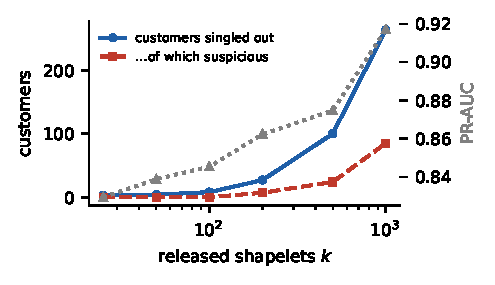
\includegraphics[width=\linewidth]{fig_sweep.pdf}\\[2pt]
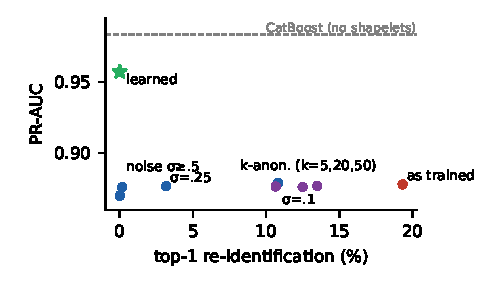
\includegraphics[width=\linewidth]{fig_tradeoff.pdf}
\caption{Top: customers uniquely exposed (and how many are flagged launderers) grow with the number of released shapelets $k$, while accuracy saturates (shapelet transform, seed 0). Bottom: privacy--utility of releases (top-1 re-identification vs.\ PR-AUC; seed mean).}
\label{fig:sweep}
\end{figure}

\section{Discussion and Limitations}
SAML-D is synthetic and activity-matched sampling makes detection optimistic; however, the leakage mechanism (copied subsequences, stored statistics) does not depend on the data. Our shapelet transform is a faithful simplification (AUC-based quality instead of information gain) because a standard implementation degenerated on our sparse series. The attack assumes the adversary's pool contains the source; consortium AML and model-sharing make this plausible. Noise and learned shapelets carry no formal guarantee; differentially private shapelet selection and DP-SGD training are natural next steps.

\textbf{Recommendations.} Treat shapelets as personal data; never release normalisation statistics; prefer learned or noised shapelets; and audit interpretable financial models with \emph{per-explanation} re-identification, not only aggregate membership inference.

\bibliographystyle{ACM-Reference-Format}
\begin{thebibliography}{12}
\bibitem{ye2009} L. Ye and E. Keogh. 2009. Time series shapelets: a new primitive for data mining. In \emph{KDD}.
\bibitem{hills2014} J. Hills, J. Lines, E. Baranauskas, J. Mapp, and A. Bagnall. 2014. Classification of time series by shapelet transformation. \emph{Data Mining and Knowledge Discovery} 28.
\bibitem{grabocka2014} J. Grabocka, N. Schilling, M. Wistuba, and L. Schmidt-Thieme. 2014. Learning time-series shapelets. In \emph{KDD}.
\bibitem{guillaume2022} A. Guillaume, C. Vrain, and W. Elloumi. 2022. Random dilated shapelet transform: a new approach for time series shapelets. In \emph{ICPRAI}.
\bibitem{minirocket} A. Dempster, D. F. Schmidt, and G. I. Webb. 2021. MiniRocket: a very fast (almost) deterministic transform for time series classification. In \emph{KDD}.
\bibitem{samld} B. Oztas, D. Cetinkaya, F. Adedoyin, M. Budka, H. Dogan, and G. Aksu. 2023. Enhancing anti-money laundering: development of a synthetic transaction monitoring dataset. In \emph{IEEE ICEBE}.
\bibitem{tertychnyi2022} P. Tertychnyi, M. Godgildieva, M. Dumas, and M. Ollikainen. 2022. Time-aware and interpretable predictive monitoring system for anti-money laundering. \emph{Machine Learning with Applications} 8.
\bibitem{fedst} Z. Liang and H. Wang. 2024. FedST: secure federated shapelet transformation for time series classification. \emph{The VLDB Journal} 33.
\bibitem{pmp} PMP: privacy-aware matrix profile against sensitive pattern inference for time series. 2023. arXiv:2301.01838.
\bibitem{shokri2021} R. Shokri, M. Strobel, and Y. Zick. 2021. On the privacy risks of model explanations. In \emph{AIES}.
\end{thebibliography}
\end{document}
